\documentclass[../../main.tex]{subfiles}

\begin{document}
In order to find God Components, we start with a high-level analysis using \textit{Designite} \citep{sharma2016designite}. Designite is a quality assessment software tool that can be used to identify numerous technical debts in your software codebase. Among which, architectural smells and including God Components. To test Designite functionality, we ran the tool on the latest version of the Tika git repository; at the time of writing \texttt{2.0.0-SNAPSHOT}. Having ran the Designite Enterprise edition, 15 God Components were identified (Figure~\ref{fig:designite/cli_analysis}).

\begin{figure}[ht]
    \centering
    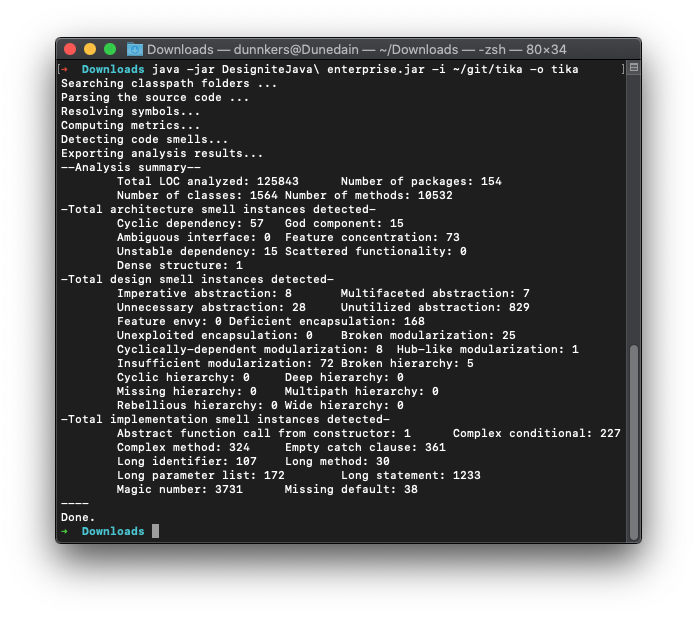
\includegraphics[width=0.8\textwidth]{report/images/designite/cli_analysis.png}
    \label{fig:designite/cli_analysis}
    \caption{Designite ran in a Terminal window. CLI shows a summary of the analysis. Extensive details of the analysis are stored in .txt files.}
\end{figure}

We can see that the codebase contains 125,843 Lines of Code (LOC) and has 10,532 methods spread over 1,564 classes packed up in 154 packages. This means the codebase is of reasonable size. Note these numbers apply only to the 2.0.0-SNAPSHOT version of the code. 

\begin{figure}[ht]
    \centering
    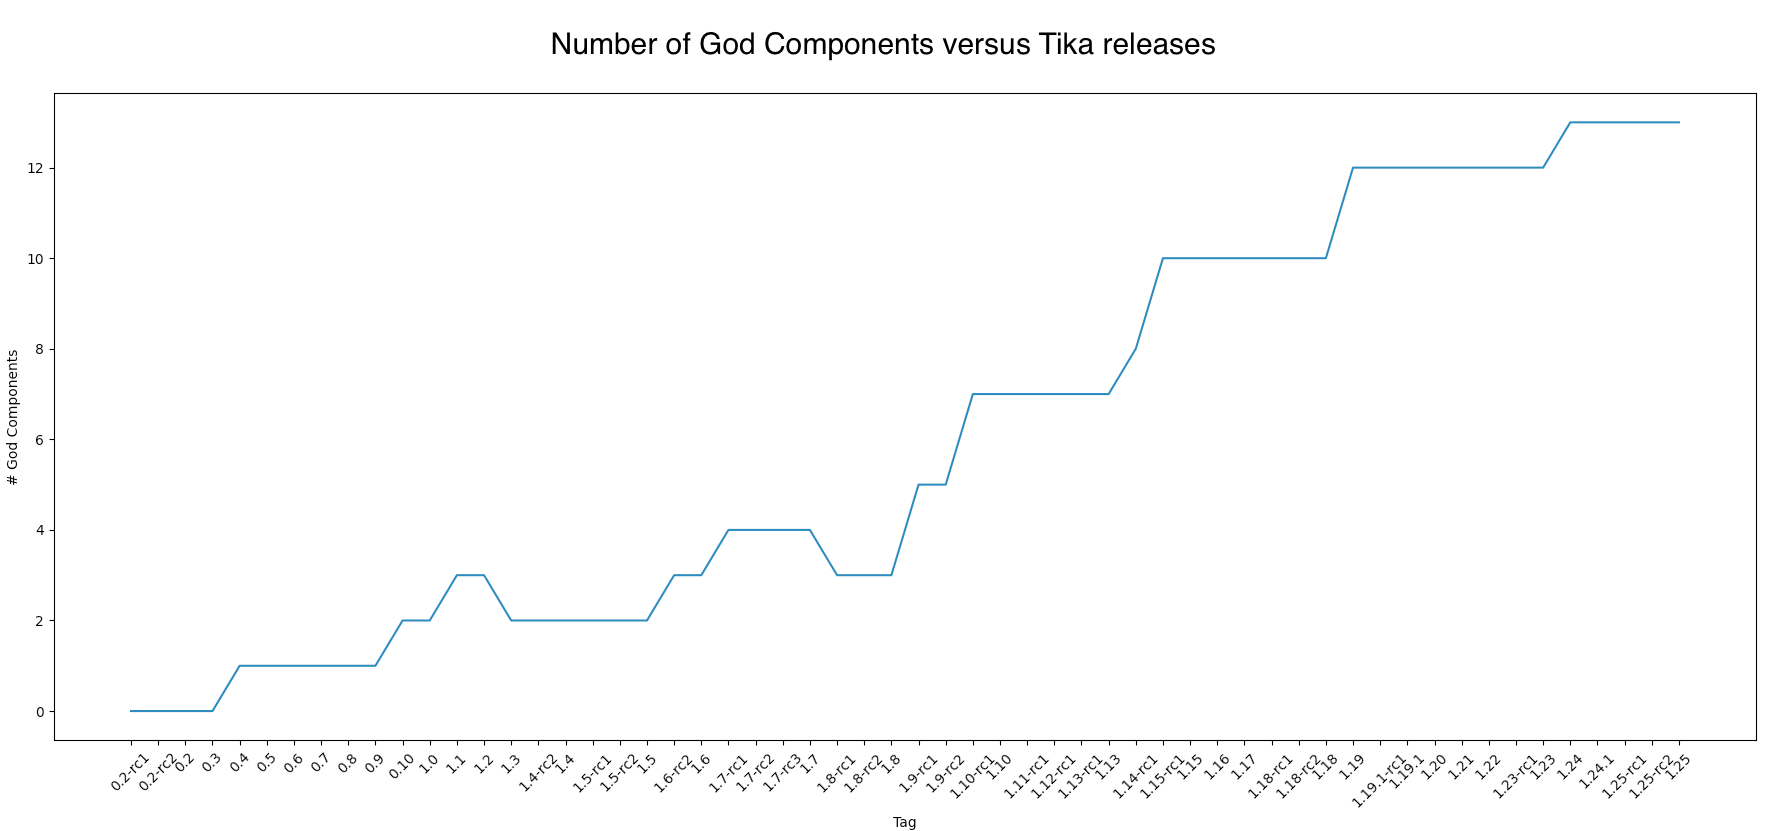
\includegraphics[width=0.8\textwidth]{report/images/designite/gcs-versus-tags.png}
    \label{fig:designite/cli_analysis}
    \caption{Designite ran in a Terminal window. CLI shows a summary of the analysis. Extensive details of the analysis are stored in .txt files.}
\end{figure}
\end{document}
